\section{Methodology}


% Descripcion del dataset
\subsection{Dataset}
\begin{frame}{Dataset}
    \begin{columns}
        \begin{column}{0.5\textwidth}
            \begin{itemize}
                \item \textbf{Vindr-mammo} Dataset \citef{phamhieuhuyVinDrMammoLargescaleBenchmark}
                \item \num{5000} digital mammogram examinations containing for each view:
                \begin{itemize}
                    \item BIRADs
                    \item Breast density
                    \item Bounding box of each finding present on the image
                \end{itemize}
                \item 10 classes of pathological findings.
                \item Bounding boxes can have multiple labels.
            \end{itemize}
        \end{column}

        \begin{column}{0.5\textwidth}
            \begin{figure}
                \centering
                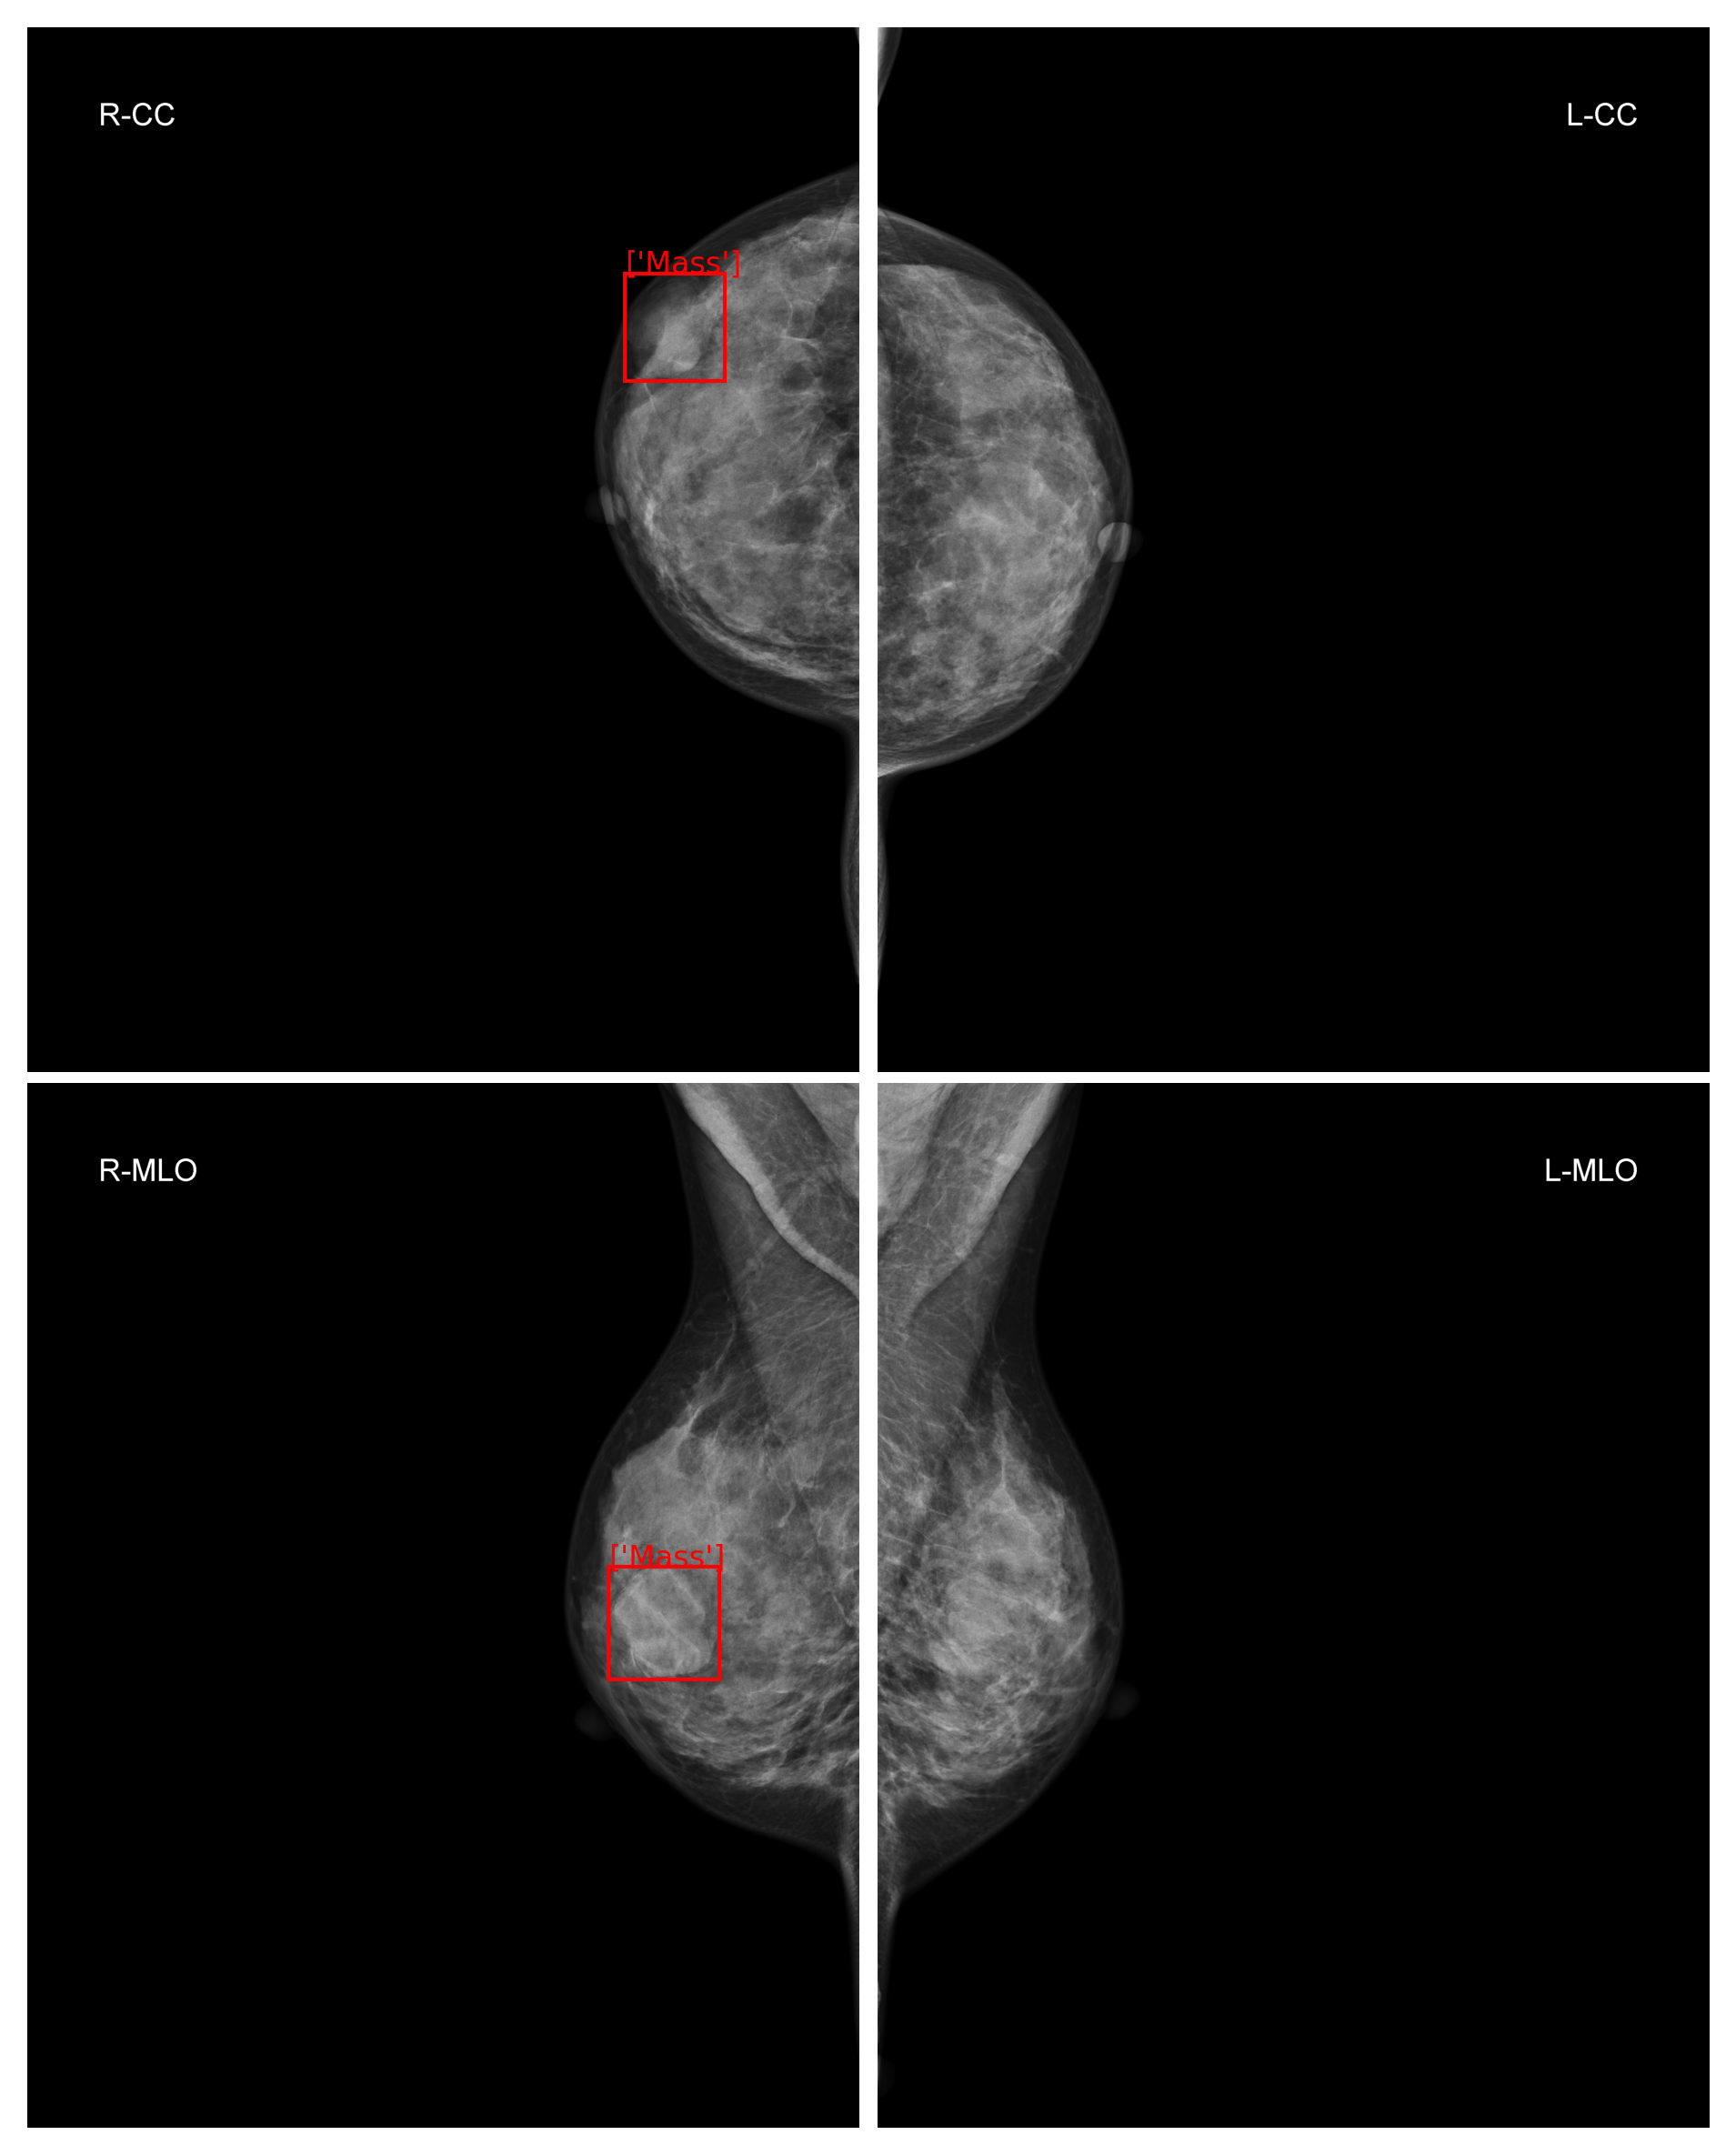
\includegraphics[height=0.7\textheight,keepaspectratio]{imagenes/vista_vindr.png}
                \caption{Example of a mammogram from the Vindr-mammo dataset.}
            \end{figure}
        \end{column}
    \end{columns}
\end{frame}

\begin{frame}{Dataset Distribution}
    % Please add the following required packages to your document preamble:
% \usepackage{booktabs}
\begin{table}[]
    \caption{Findings statistics of Vindr-Mammo Dataset}
    \label{tab:vindr-samples}
    \begin{tabular}{@{}l S[table-format=3]S[table-format=3]S[table-format=4]@{}}
    \toprule
    Finding                           & {Training} & {Test} & {Total} \\ \midrule
    Mass                              & 989      & 237  & 1226  \\
    Suspicious Calcification          & 428      & 115  & 543   \\
    Asymmetries (Global, Focal, etc.) & 313      & 79   & 392   \\
    Architectural Distortion          & 95       & 24   & 119   \\
    Skin Thickening                   & 45       & 12   & 57    \\
    Retraction (Skin or Nipple)       & 45       & 10   & 55    \\
    Suspicious Lymph Node             & 46       & 7    & 37    \\ \bottomrule
    \end{tabular}
    \end{table}
\end{frame}

% Procesamiento de imagenes
\subsection{Image Processing}

\begin{frame}{Image Processing Pipeline}
    \begin{itemize}
        \item Each DICOM Image is normalised to a range of $[0, 1]$
        \item Apply CLAHE algorithm \citef{pizerContrastlimitedAdaptiveHistogram1990} for histogram equalization at 2 different scales
        \item Fuse the equalized images with the original, channel-wise
        \item Image is cropped to the bounding box of the breast using Otsu's thresholding.
    \end{itemize}
\end{frame}

\begin{frame}[plain]
    \begin{figure}
        \centering
        \includegraphics[height=0.9\textheight]{imagenes/improcessingV2.png}
        \caption{Image processing pipeline}
    \end{figure}
\end{frame}
% Seleccion de nuestro modelo
\subsection{Model Selection}
\begin{frame}{Evaluation of deep learning architectures}
    We evaluated the following architectures as a backbone:
    \begin{itemize}
        \item ResNet50
        \item EfficientNetV2 \cite{tanEfficientNetV2SmallerModels2021}
        \item DenseNet
        \item Swin Transformer
        \item MobileNet
        \item VGG19
    \end{itemize}

    Classifier Layer using 2 layer MLP with \num{512} hidden units and ReLU activation.
    Output layer with 10 units and sigmoid activation.
\end{frame}

% Modelo de extraccion de caracteristicas
\begin{frame}{Feature Extraction Model}
    \begin{itemize}
        \item We use the backbone of the selected architecture as a feature extractor.
        \item The output of the backbone is flattened and fed to the classifier.
        \item The classifier is trained using the cropped images.
    \end{itemize}
\end{frame}

\subsection{Training}
\begin{frame}{Image Sampling}
    \begin{itemize}
        \item For each finding present on an image, we sampled a random area of the finding.
        \item Area and aspect ratio randomly sampled from an Uniform distribution.
        \begin{itemize}
            \item Area: $[.05, 5.]$ of the finding bounding box area.
            \item Aspect ratio: $[0.33, 1.66]$ of the finding bounding box aspect ratio.
            \item The bounding box center is uniform sampled from \SI{50}{\pixel} around the original center.
        \end{itemize}
        \item For normal images (\emph{No Finding}), we sample a random area of the breast, with similar sampling parameters.
        \item Sampled image is resized to $256 \times 256$ pixels.
        \item \textbf{Image augmentation}: Contrast, brightness, saturation, flip and rotation are randomly modified.
    \end{itemize}
\end{frame}

\begin{frame}{Example of sampling}
    \begin{figure}
        \centering
        \includegraphics[height=0.7\textheight,keepaspectratio]{imagenes/pos_proposals.png}
        \caption{Example of sampling of ten positive proposals from a finding.}
    \end{figure}
\end{frame}

\begin{frame}{Training parameters}
    \begin{itemize}
        \item Focal Loss Function \begin{equation*}
            \mathcal{L}_{\text{Focal}} = -(1 - p_t)^\gamma \log{(p_t)}
        \end{equation*}
        \item Adam Optimizer with a starting learning rate of \num{1e-4}
        \item Reduce on plateau with a patience of 5 epochs and a factor of \num{0.1}
        \item Weighted sampling of the dataset, in order to reduce imbalance.
    \end{itemize}
\end{frame}

% Analisis mediante ventans
\subsection{Sliding patches for detection}
\begin{frame}{Local Information}
    
\end{frame}

\begin{frame}{Our method}
    \begin{itemize}
        \item Segmentation of the complete image into a set of overlapping windows of size $256 \times 256$ pixels and stride of \SI{32}{\pixel}.
        \item Reconstruction of prediction heatmap from the overlapping windows.
    \end{itemize}
\end{frame}
